\documentclass[letterpaper, 10 pt]{report}

\usepackage{graphicx}
\usepackage{color}
\usepackage{hyperref}
\hypersetup{
    colorlinks,
    linktoc=all,
    citecolor=black,
    filecolor=black,
    linkcolor=black,
    urlcolor=black
}


\graphicspath{{./Pictures/}}
\usepackage{array}


\usepackage{chngcntr}
\counterwithout{section}{chapter}
\usepackage{listings}




% -------------------------------------------------------------------------------------
% BEGIN DOCUMENT
% -------------------------------------------------------------------------------------
\begin{document}
\title{Hexapod User Manual}
\author{Dan Thilderkvist \and Sebastian Svensson}
\maketitle
\pagestyle{empty}

% -------------------------------------------------------------------------------------
% TABLE OF CONTENTS
% -------------------------------------------------------------------------------------
\tableofcontents
\newpage

% -------------------------------------------------------------------------------------
% INTRODUCTION
% -------------------------------------------------------------------------------------
\section{Introduction}
This documentation contains an overview of the Simulink files and hardware of the Phantom Hexapod Mark II.
In some of the Simulink files there are more detailed comments.


\section{Requierd toolboxes}
The following toolboxes and support package are required to run the model.

\begin{itemize}
\item Embedded Coder
\item Simulink Coder
\item Embedded Coder Support Package for BeagleBone Black Hardware 
\item Matlab
\item SimMechanics
\item Simscape
\item Simulink
\item Instrument Control Toolbox
\end{itemize}



\section{Run Instructions}
Using the thesis work might not be totally self explanatory.
Here follows a couple of walk-through sections on how to use the different parts.
First thing to do in every scenario is to run the init{\_}script.m.
This ensures that folders are added to the MATLAB workpath.

\subsection{Running hexapod Model}
For running the hexapod as a model the file Control/DevelopmentModel.slx can be used.
This file contains a Model of the hexapod built up by the different library files and a controller built up similarly.
Running the combination of the two is done by basically pressing play and SimMechanics should provide visual results.
If there is a desire to change the hard-coded input to the controller one can change this inside the controller block 2 levels down.
All changes to main controller and IK should be avoided inside this file.
Those changes are better done in the library files.

\subsection{Running Code Generation to the hexapod}
First assemble the power to the hexapod.
Connect the battery to the battery voltage monitor device to be able to monitor battery voltage.
The monitor device will beep temporary when connected.
When battery voltage is to low the device will start beeping continuously (charge the battery).
Also connect the battery to the connection bringing power to BeagleBone Black, ArbotiX and servos.
The BeagleBone gets powered directly but in order to power ArbotiX and servos the switch on the back of the hexapod has to be switched.

Start the file Control/CodeGenerationSetup.slx.
This files provide two options, run in external mode or deploy to hardware.
Running in external mode (play button) provides the ability to monitor signals with scopes in Simulink but needs the BeagleBone connected to the computer by USB.
Deploy to hardware (blue deploy button) allows for no wire connection but do not supply scope data.

Power on the remote first after the code has started running to avoid communication being off-sync.
When deployed to hardware the script StartBB and StopBB can be used to start/stop the program without having to recompile code.

\newpage
\subsection{Using the remote}

A picture of the remote can be seen in Figure \ref{fig:commander}.
Description of each button is described in Table \ref{tab:remotecontroll}.



\begin{figure}[h!]%float objekt h-här h!-verkligen här t-toppen
\centering%centrerar bilden på sidan
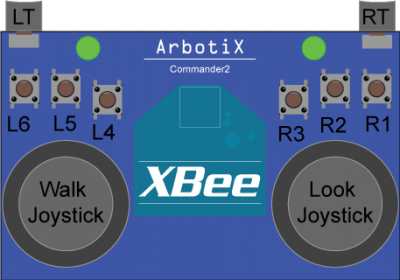
\includegraphics[width=0.7\textwidth]{Commander.png}%0.9 textbredder
\caption{Location on the different controls on the remote.}%skapa bildtext
\label{fig:commander}%tag label på bilden
\end{figure}


\setlength{\extrarowheight}{5pt}
%%Command for writing data to all of the servos
\begin{table}[h!]
\centering%centrerar bilden på sidan
\begin{tabular}{|l|l|}
\hline Name 					&   Description			\\ 
\hline WalkH $\leftrightarrow$	& 	Strafe left/right	\\ 
\hline WalkV $\updownarrow$ 	&   Move forward/back 	\\ 
\hline LookH $\leftrightarrow$	& 	Rotate left/right 	\\  
\hline LookV $\updownarrow$		&   N/A					\\ 
\hline LT&      Lower the body		\\
\hline RT& 	    Rise the body		\\  
\hline L6&      Normal walking		\\ 
\hline L5&      Experimental walk patterns with constraints\\
\hline L4&      N/A					\\
\hline R3& 	    N/A					\\  
\hline R2&      N/A					\\ 
\hline R1&      Balancing mode    	\\
\hline 
\end{tabular} 
\caption{Description of the remote control.}%skapa bildtext
\label{tab:remotecontroll}%tag label på bilden
\end{table}



% -------------------------------------------------------------------------------------
% Control
% -------------------------------------------------------------------------------------

\section{Control}
\label{sec:control}
The control-structure is described in the master thesis report.
Here most of the control files will be described.

The full system is triggered by a trigger-system in order to keep control of execution order.
The trigger system is saved as a library and linked to from the various implementations.
Trigger system library can be found under Simulink{\_}Lib/Control.
Here is also the rest of the control libraries located.
IK, MainController, coordinate translater and a test sequence exists.
The most advanced one of these is the main controller.
If development of the controller is to be done it is inside this it can be performed.
The controller implementation utilizes written m-files.
These are located at Control/MatlabFunctions and are explained by comments in the code.

There is a folder located as Control/LegConstriants.
The script inside is used to get a visualization of the constraint boundaries that can be used for the legs. 
Script is hopefully self explanatory.

% -------------------------------------------------------------------------------------
% Documents
% -------------------------------------------------------------------------------------
\section{Documents}
This folder contains documentation for the different electrical components and other important parts of the hexapod.
\begin{description}
  \item[ArbotiX-M] documentation the arduino card ArbotiX-M 
  \item[Beaglebone black] documentation the BeagleBone Black
  \item[IMU] documentation for MPU9150
  \item[Movies] contains movies of Simulink models running on hardware and in simulation
  \item[Servo manual]  contains documentation on the AX12A servos
  \item[ThesisManual] contains .tex files to expand and rebuild this manual
  \item[ThesisDocuments] contains popular summary,thesis report and a presentation 
\end{description}

% -------------------------------------------------------------------------------------
% Measurements
% -------------------------------------------------------------------------------------
\section{Measurements}
This folder contains some code for running step responses on the AX12A servos. 
To use this files, load \texttt{StepTest.ino} onto the ArbotiX card using Arduino IDE.
Open the file \texttt{TestSetup.slx} and select the com port to which the ArbotiX card is connected. 
Finally set parameters for the step test in \texttt{testSetupRun.m} and run the script.
Data will be logged by the ArbotiX card and then saved in a folder structure on the PC.

% -------------------------------------------------------------------------------------
% Model
% -------------------------------------------------------------------------------------
\section{Model}

\subsection{CAD/Hexapod}
The folder \texttt{Cad export} contains the file produced by SimMechanics Link and are used for visualization of the hexapod inside of Simulink.

The folder \texttt{SolidWorks} contains the SolidWork parts and assembly files to construct the hexapod.
\texttt{Common leg parts} contains parts to assemble  the three leg parts (coxa, femur and tibia).
The two folders \texttt{Left leg} and \texttt{Right leg} contains coxa, femur and tibia part for each leg.
The difference between those files are the placement of the servos.
 
To update mass of the parts first open the part file and check were the extra coordinate system are located. 
Then open the corresponding assembly file and perform the update needed.
Choose Edit->rebuild 
Goto File->Save as->.part and select All components.
Open the part file and insert the coordinate system.
Finally use SimMechanics link to export the updated file to SimMechanics.
If only the mass of the part needs to be changed this can be done directly in SimMechanics.

The file Hexapod.sldasm contains the complete hexapod to export into SimMechanics. 
The legs and joints are added when the model have been imported into SimMechanics.


\subsection{Contact{\_}force}
This folder contains work done to model contact forces in SimMechanics.
\texttt{Left{\_}LegGCfriction.slx} shows a demonstration of contact with floor for one hexapod leg using SimMechanics contact force library.
\texttt{hexapod{\_}with{\_}floor.slx} contains the complete hexapod with six feet contact points with the floor.
the contact point are placed at the center of each foot \texttt{F{\_}GC}.
Other approaches for modelling contact forces are presented in the folder \texttt{Other approaches}.
Some useful links to use when modelling contact forces can be found at 
\url{http://www.mathworks.com/matlabcentral/fileexchange/49374-rolling-ball-on-plane}
and
\url{http://www.mathworks.com/matlabcentral/fileexchange/47417-simmechanics-contact-forces-library}.


% -------------------------------------------------------------------------------------
% Simulink_Lib
% -------------------------------------------------------------------------------------
\newpage
\section{Simulink{\_}Lib}
This folder contains library files to construct the hexapod inside Simulink and SimMechanics. 
The file \texttt{Custom{\_}buses.mat} contains definitions for the different buses used in the Simulink models.
\subsection{BeagleBoneBlack}
\begin{description}
\item[IMU{\_}DMP] contains documentation and code for using the DMP on MPU9150
\item[Test] contains files for testing the various S-Function builder blocks
\item[Working Code] contains the code generated for the S-Function Builder blocks 
\item[BeagleBoneBlackCom.slx] contains all S-Function Builder blocks for use on the BeagleBone Black
\item[ServoCommand.slx] contains blocks to build up a message to send position references to the servos using the write to servo block found in \texttt{BeagleBoneBlackCom.slx}
\end{description}


\subsection{How to build a S-Function}
Set the working folder in MATLAB to were the generated code ends up e.g. to build the commander block select \texttt{WorkingCode\textbackslash Commander}.

\begin{enumerate}
\item Open the S-Function Builder goto Build Info tab-> Additional methods select Terminate.
\item Press build in the upper right corner.
\item Open the generated \texttt{*{\_}wrapper.c} goto the end of the file and copy the line \texttt{close(xbee{\_}fd);}.
\item Open the \textit{SFunctionName}.c and insert the line inside the 
\texttt{static void mdlTerminate(SimStruct *S)} function.
\end{enumerate}

When building the IMU{\_}DMP make sure to update \texttt{Libraries tab} with correct path to include existing source code.

\newpage
\subsection{Note on using UART}
To make the UART work the following changes have to be made to \texttt{uEnv.txt} found in 
\texttt{BeagleBone Getting Started (F:)} on the BeagleBone Black.
Before:
\begin{lstlisting}[frame=single,numbers=left,breaklines=true,firstnumber=17]
##WIP: v3.13+ capes..
#cape=lcd4-01
#cape=

##note: the eMMC flasher script relies on the next line
mmcroot=UUID=5338fca0-6bf1-4297-8feb-a7a909cad7a2 ro
mmcrootfstype=ext4 rootwait fixrtc
\end{lstlisting}

After:
\begin{lstlisting}[frame=single,numbers=left,breaklines=true,firstnumber=17]
##WIP: v3.13+ capes..
#cape=lcd4-01
#cape=

#Setup serial ports
optargs=capemgr.enable_partno=BB-UART1,BB-UART2,BB-UART3,BB-UART4,BB-UART5


##note: the eMMC flasher script relies on the next line
mmcroot=UUID=5338fca0-6bf1-4297-8feb-a7a909cad7a2 ro
mmcrootfstype=ext4 rootwait fixrtc
\end{lstlisting}



















\subsection{Control}
This files are described in \ref{sec:control}.

\subsection{Model}
\begin{description}
\item[Completemodels.slx] contains model which are controlled by either torque or position. Also contains a experimental model for use ballonfloor contact force model see \url{http://www.mathworks.com/matlabcentral/fileexchange/49374-rolling-ball-on-plane}.
\item[Servo model] contains models for the AX12A servos. Two models are present one for torque and one for position actuation. 
\item[HexapodLib] contains models of the different parts of the hexapod. Two models are present one for torque and one for position actuation.
The interface blocks are used to connect the input signal to the correct servo id. Check the simulation model to get a example.
\end{description}


\subsubsection{SM{\_}Contact{\_}Forces{\_}Lib}

A download of the contact forces library found at \url{http://www.mathworks.com/matlabcentral/fileexchange/47417-simmechanics-contact-forces-library}.



% -------------------------------------------------------------------------------------
% Software
% -------------------------------------------------------------------------------------
\section{Software}

%TODO skriv vad de andra delarna används till
\begin{description}
\item[Arduino{\_}Phoenix{\_}Parts-master] A more advanced program for running the  hexapod. 
More information can be found at 
\url{http://learn.trossenrobotics.com/10-interbotix/crawlers/phantomx-hexapod/68-phoenix-code.html}
\item[HexapodMKIICommander-master] contains the code delivered with the hexapod
\item[PosePrograms] contains a program for recording and playing back different poses for the hexapod.
More information can be found at 
\url{http://learn.trossenrobotics.com/8-arbotix/131-dynapose-dynamixel-arbotix-pose-tool.html}
\item[VirtualCommander] A program that emulates the remote to the hexapod.
More information can be found at 
\url{http://learn.trossenrobotics.com/projects/145-virtual-commander-generic-software-robot-control.html}.
\end{description}



% -------------------------------------------------------------------------------------
% REFERENCES
% -------------------------------------------------------------------------------------
%\bibliography{}

% -------------------------------------------------------------------------------------
% END DOCUMENT
% -------------------------------------------------------------------------------------
\end{document}